% This is "sig-alternate.tex" V2.0 May 2012
% This file should be compiled with V2.5 of "sig-alternate.cls" May 2012
%
% This example file demonstrates the use of the 'sig-alternate.cls'
% V2.5 LaTeX2e document class file. It is for those submitting
% articles to ACM Conference Proceedings WHO DO NOT WISH TO
% STRICTLY ADHERE TO THE SIGS (PUBS-BOARD-ENDORSED) STYLE.
% The 'sig-alternate.cls' file will produce a similar-looking,
% albeit, 'tighter' paper resulting in, invariably, fewer pages.
%
% ----------------------------------------------------------------------------------------------------------------
% This .tex file (and associated .cls V2.5) produces:
%       1) The Permission Statement
%       2) The Conference (location) Info information
%       3) The Copyright Line with ACM data
%       4) NO page numbers
%
% as against the acm_proc_article-sp.cls file which
% DOES NOT produce 1) thru' 3) above.
%
% Using 'sig-alternate.cls' you have control, however, from within
% the source .tex file, over both the CopyrightYear
% (defaulted to 200X) and the ACM Copyright Data
% (defaulted to X-XXXXX-XX-X/XX/XX).
% e.g.
% \CopyrightYear{2007} will cause 2007 to appear in the copyright line.
% \crdata{0-12345-67-8/90/12} will cause 0-12345-67-8/90/12 to appear in the copyright line.
%
% ---------------------------------------------------------------------------------------------------------------
% This .tex source is an example which *does* use
% the .bib file (from which the .bbl file % is produced).
% REMEMBER HOWEVER: After having produced the .bbl file,
% and prior to final submission, you *NEED* to 'insert'
% your .bbl file into your source .tex file so as to provide
% ONE 'self-contained' source file.
%
% ================= IF YOU HAVE QUESTIONS =======================
% Questions regarding the SIGS styles, SIGS policies and
% procedures, Conferences etc. should be sent to
% Adrienne Griscti (griscti@acm.org)
%
% Technical questions _only_ to
% Gerald Murray (murray@hq.acm.org)
% ===============================================================
%
% For tracking purposes - this is V2.0 - May 2012

\documentclass{sig-alternate}
\usepackage{fixltx2e,algpseudocode,pifont,graphicx}
\usepackage[linesnumbered,ruled,vlined]{algorithm2e}
\algrenewcommand\Return{\State \algorithmicreturn{} }%

\begin{document}
%
% --- Author Metadata here ---
\conferenceinfo{WOODSTOCK}{'97 El Paso, Texas USA}
%\CopyrightYear{2007} % Allows default copyright year (20XX) to be over-ridden - IF NEED BE.
%\crdata{0-12345-67-8/90/01}  % Allows default copyright data (0-89791-88-6/97/05) to be over-ridden - IF NEED BE.
% --- End of Author Metadata ---

\title{Spatial Alarms in the Obstructed Space\titlenote{(For use with
SIG-ALTERNATE.CLS. Supported by ACM.}}
%\subtitle{[Extended Abstract]
%\titlenote{A full version of this paper is available as
%\textit{Author's Guide to Preparing ACM SIG Proceedings Using
%\LaTeX$2_\epsilon$\ and BibTeX} at
%\texttt{www.acm.org/eaddress.htm}}}
%
% You need the command \numberofauthors to handle the 'placement
% and alignment' of the authors beneath the title.
%
% For aesthetic reasons, we recommend 'three authors at a time'
% i.e. three 'name/affiliation blocks' be placed beneath the title.
%
% NOTE: You are NOT restricted in how many 'rows' of
% "name/affiliations" may appear. We just ask that you restrict
% the number of 'columns' to three.
%
% Because of the available 'opening page real-estate'
% we ask you to refrain from putting more than six authors
% (two rows with three columns) beneath the article title.
% More than six makes the first-page appear very cluttered indeed.
%
% Use the \alignauthor commands to handle the names
% and affiliations for an 'aesthetic maximum' of six authors.
% Add names, affiliations, addresses for
% the seventh etc. author(s) as the argument for the
% \additionalauthors command.
% These 'additional authors' will be output/set for you
% without further effort on your part as the last section in
% the body of your article BEFORE References or any Appendices.

\numberofauthors{3} %  in this sample file, there are a *total*
% of EIGHT authors. SIX appear on the 'first-page' (for formatting
% reasons) and the remaining two appear in the \additionalauthors section.
%
\author{
% You can go ahead and credit any number of authors here,
% e.g. one 'row of three' or two rows (consisting of one row of three
% and a second row of one, two or three).
%
% The command \alignauthor (no curly braces needed) should
% precede each author name, affiliation/snail-mail address and
% e-mail address. Additionally, tag each line of
% affiliation/address with \affaddr, and tag the
% e-mail address with \email.
%
% 1st. author
\alignauthor
Md. Touhiduzzaman\\
       \affaddr{Department of Computer Science}\\
       \affaddr{Bangladesh University of Engineering and Technology}\\
       \affaddr{Dhaka,Bangladesh}\\
       \email{tz08128@gmail.com}
% 2nd. author
\alignauthor
Sezana Fahmida \\
       \affaddr{Department of Computer Science}\\
       \affaddr{Bangladesh University of Engineering and Technology}\\
       \affaddr{Dhaka,Bangladesh}\\
       \email{sezanafahmida@gmail.com}
% 3rd. author
\alignauthor
Tanzima Hashem \\
       \affaddr{Department of Computer Science}\\
       \affaddr{Bangladesh University of Engineering and Technology}\\
       \affaddr{Dhaka,Bangladesh}\\
       \email{tanzimahashem@gmail.com}
%\and  % use '\and' if you need 'another row' of author names
% 4th. author
%\alignauthor Lawrence P. Leipuner\\
 %      \affaddr{Brookhaven Laboratories}\\
  %     \affaddr{Brookhaven National Lab}\\
   %    \affaddr{P.O. Box 5000}\\
    %   \email{lleipuner@researchlabs.org}
% 5th. author
%\alignauthor Sean Fogarty\\
 %      \affaddr{NASA Ames Research Center}\\
  %     \affaddr{Moffett Field}\\
   %    \affaddr{California 94035}\\
    %   \email{fogartys@amesres.org}
% 6th. author
%\alignauthor Charles Palmer\\
 %      \affaddr{Palmer Research Laboratories}\\
  %     \affaddr{8600 Datapoint Drive}\\
   %    \affaddr{San Antonio, Texas 78229}\\
    %   \email{cpalmer@prl.com}
}
% There's nothing stopping you putting the seventh, eighth, etc.
% author on the opening page (as the 'third row') but we ask,
% for aesthetic reasons that you place these 'additional authors'
% in the \additional authors block, viz.
%\additionalauthors{Additional authors: John Smith (The Th{\o}rv{\"a}ld Group,
%email: {\texttt{jsmith@affiliation.org}}) and Julius P.~Kumquat
%(The Kumquat Consortium, email: {\texttt{jpkumquat@consortium.net}}).}
%\date{30 July 1999}
% Just remember to make sure that the TOTAL number of authors
% is the number that will appear on the first page PLUS the
% number that will appear in the \additionalauthors section.

\maketitle
\begin{abstract}
Spatial Alarms are personalized Location Based service(LBS), that are triggered by a specific location of a moving user, instead of time. In this paper, we introduce an efficient algorithm to evaluate spatial alarm queries in obstructed space. Existing work in this area has focused mainly on Euclidean distance and road network models. The key idea of our approach is to compute a specific region within which the answer set of our query remains unchanged. Our aim is to reduce redundant computations in client side, while preserving the accuracy of the alarms triggered.
\end{abstract}

% A category with the (minimum) three required fields
\category{H.4}{Information Systems Applications}{Miscellaneous}
%A category including the fourth, optional field follows...
\category{D.2.8}{Software Engineering}{Metrics}[complexity measures, performance measures]

\terms{Theory}

\keywords{Spatial Alarm, Obstructed Space}
%\theoremstyle{plain}
\newtheorem{thm}{Theorem}[section] % reset theorem numbering for each chapter

%\theoremstyle{definition}
\newtheorem{defn}[thm]{Definition} % definition numbers are dependent on theorem numbers
\newtheorem{exmp}[thm]{Example} % same for example numbers

\section{Introduction}
The widespread use of smart phones has led to the proliferation of LBSs. %According to many, the next step in location based services is Spatial Alarms. Many believe this particular feature is going to dominate the future mobile-phone computing systems./%
Starting from static LBS(Location Based Service) such as finding the nearest pharmacy for a user's location, now-a-days LBSs are tailored for moving users. Spatial Alarms are an important class of LBS,that are triggered by a specific location of a moving user, irrespective of time. "Remind me if I'm within 100 meters of a pharmacy" is a possible example of a spatial alarm.
% It is a personalized LBS which can vary from user to user.\\

Existing work in this area has focused mainly on Euclidean distance and Road Network models \cite{bamba},\cite{roadalarm},\cite{liu}. However, Spatial alarm evaluation in the obstructed space is different than road network or Euclidean space as it considers the obstacles in the path to the location of alarm. It is better approximated by a pedestrian scenario while road networks are approximated by vehicle scenarios. A pedestrian's path is not limited by roads. However, a pedestrian is obstructed by various obstacles such as buildings or trees. Thus while calculating the distance from alarms, we have to consider the obstructed distance\cite{deberg}. In this paper we propose a unique approach to evaluate spatial alarms in obstructed space. To the best of our knowledge this query has not been addressed in any existing research work.
%It is noteworthy that spatial alarms are quite dissimilar to spatial range query. 

Spatial alarms are based on a predefined location with a given alarming zone radius thus applying the techniques that are used in answering spatial range queries is both inefficient and wasteful as, in spatial range query continuous re-evaluation of user's location is needed in case of a mobile user. However,in spatial alarm, the user's location is not relevant at all times. If we start to evaluate spatial alarms as soon as the user is on the move even if the user is far away from her desired location our efforts will be futile. Another  challenge in spatial alarm processing is the communication cost between the server and the client.

The key idea of our approach is to calculate a dynamic \textit{safe region}, within which no computation has to be done to provide an accurate alarm trigger. We will use an R-tree structure to index both obstacles and POI's in our approach. Our spatial alarm processing system has two different modes for efficient and effective processing of spatial alarms,namely, Bandwidth saving mode and Computational Cost Saving mode. Our approach accounts for both accuracy and efficiency by focusing on (1) No alarms being missed in user's proximity (2) Avoiding wasteful computation in client side (3) minimizing data transfer between server and client. In summary the our main contributions are: 
\begin{itemize}
\setlength\itemsep{0em}
\item We introduce an efficient algorithm for evaluation of spatial alarm queries in obstructed space.
\item We provide a spatial alarm evaluation system for mobile user.
\item We provide an algorithm to calculate a dynamically changing region to accurately evaluate spatial alarm queries without any computation.
\item We provide an extensive experimental analysis to compare the accuracy of our approach with other naive approaches based on different parameters.
\end{itemize}


\section{Problem Setup}
Existing research has categorized spatial alarms into three types: public, shared and private. Public alarms are alarms which are active for every user within the system, such as an alarm must be sent to everyone within 100 meters of a building on fire. Private alarms are user defined alarms which can be viewed by the user, such as a user might set an alarm to alert her if she is within 100 meters of her favorite coffee shop. Shared alarms are shared between specific groups of people. In the previous example if a user chooses to share the alarm for the coffee shop with some of her friends it becomes a shared spatial alarm.\\
In \cite{bamba} spatial alarms has been categorized into three different types: 1)moving subscriber with static target, 2) static subscriber with moving target 3) moving subscriber with moving target. In this paper we are only considering the first type, that is moving subscriber with static target. 
In \cite{mur} spatial alarms have been approximated by rectangular bounding box, in our approach we are considering the spatial alarm region as a circle with radius r.\\ \\
\textit{Obstructed Space Path Problem} \cite{ognn} denotes the problem of finding the shortest route between two query-points  in Obstructed Space where non-intersecting 2D polygons represent \textit{obstacles} and where the route does not traverse through any obstacles. The length of the Obstructed route between points a and b is called the \textit{Obstructed Distance} between a and b, denoted by $dist_o(p_i,q)$.\\ \\
A \textbf{Spatial Alarm Query in Obstructed Space} is formally defined as follows:
%\begin{defn}
Given a moving query point q and a range r for an alarm, a Spatial Alarm Query returns $\forall p_i \in P=\left\lbrace p_1,p_2,p_3...p_n\right\rbrace  $ which have $dist_o(p_i,q)<r $
%\end{defn}
% The GETALLPOI(R,P) and GETOBSTACLESET(q,R,O) functions populates the sets P and O with the POIs and obstacles respectively within the distance R from the client's current location.
%\\MAKEVISGRAPH(P,O) returns the \textit{visibility graph} V$_G$ with the set of POIs P and Obstacles O.
%A \textbf{Visibility Graph} is a graph $V_G(V,E)$ where each v $\in$ V is either a POI or a Data point and for each (u,v)$ \in$ V, there is an edge e between u and v if and only if it does not interesect with any obstacles i.e. u and v are \textit{visible} to each other. \\
%EUCLIDEANDIST(q1,q2) returns the euclidean space distance between two points q1 and q2.\\
%CHECKNEWPOI(q,$r_k$,P) \\
%ALARMUSER(P$_i$) triggers an alarm to the user for the alarm $P_i$. \\  
% Single-column table

\section{Preliminaries}
Spatial alarms are location-based, user-defined triggers which will possibly shape the future mobile application computations. They are distinct from spatial range query and do not need immediate evaluation after the user has activated them. The spatial alarm evaluation strategies are judged based on two features, correctness and scalability. Correctness refers to the quality that guaranties no alarms are missed. And scalability is the feature that measures the number of POI's the system can adapt to. 
In this paper, We propose a novel approach to evaluate spatial alarms in obstructed space which ensures both high accuracy and high scalability.

We define three different type of regions: \textit{Known Region},\textit{Reliable Region} and \textit{Safe Region}\\ \\

\textbf{Known Region:} We define two different known regions for the POIs and the obstacles. The region containing at least 1 POI is the known region for POI.\\
The region circulating the POIs known region containing none or single colliding obstacles is the known region for the obstacles. The set of obstacles and POIs within this region is known to the client. 
Both of the known regions are represented by a parabola whose focus point is the users location q,with the equation $y^2=4ax$ where $a=mr$ which are bounded by a straight line. \\ \\


\textbf{Reliable Region:} Within which region, no further query to the server has to be done to compute a consistent set of answers, that is termed as a reliable region. The reliable region is also a parabolic region bounded by a straight line,where each bounding point of the parabolic curve is at a distance r from the known regions parabolic curve. $ \forall p_i=(x,y) $ in the known region, $ \forall p_j=(x_r,y_r) $ in the reliable region, $ dist_E(p_i,p_j)\geq r $ By this definition no further queries to the server has to be done to compute a consistent set of answers. Because, for any $q =p_j dist_E(q,p_j) \geq r$ where $p_j$ is a point on the boundary of the reliable region. And for all other points $ p_i $ inside the reliable region $  dist_E(q,p_i)>r$ \\ \\


\textbf{Safe Region:} A safe region is the region located inside reliable region within which the answer set of POIs remains unchanged for a moving client. We will denote the radius of the safe region as $r_{safe}$. Given the user's previous location $P_1$ and the current location $P_2$, if $(P_1 - P_2) < r_{safe}$, then no recalculation is needed to compute the answer. If the safe region surpasses the reliable region at some points 
\\ \\

\begin{table}[h]
\centering 

\caption{Symbol Table}
\begin{tabular}{|c|c|} \hline
Symbols&Meaning \\ \hline
P & Set of POIs\\ \hline
O & Set of Obstacles\\ \hline
q & Location of user\\ \hline
$r$ & Alarming range\\ \hline
$V_{G}$       & Visibility Graph\\ \hline
$dist_E$(p,q) & Euclidean distance between points p and q\\ \hline
$dist_O$(p,q) & Obstructed distance between points p and q\\ \hline
$r_{safe}$    & Radius of safe region\\ \hline
$m$           & Real number in the range $[2,\infty)$ \\ \hline
$n$           & Real number in the range $[1,\infty) $  \\ \hline
$\theta_i $   & Angle between consecutive path segments \\ \hline 
$ S $         & Users path history as a set of straight lines \\ \hline
$(m_i,c_i,l_i)$ & A line with slope $m_i$, intercept $c_i$ and length $l_i$ \\ \hline

\end{tabular}
\end{table}

 
\section{Related Work}
\subsection{Spatial Alarms}
Extensive research has been performed and various  effective algorithms have been proposed \cite{roadalarm},\cite{mur},\cite{bamba} to process spatial alarms in Euclidean space and road network in recent years. Euclidean space considers the straight line distance between two points irrespective of obstacles on the other hand in road networks navigation is limited along predefined roads. \cite{roadalarm}proposes a solution to the spatial alarm problem for moving users on road network. They introduce road network-based spatial alarms using segment length-based and travel time-based road network distances. Our approach aims to provide a solution to the same problem, depicted in an obstructed space\cite{deberg} scenario. Again, their solution incorporates the concept of hibernation time, a time during which no processing takes place in the mobile client or the processing engine comprehensive research, where in our approach we propose the novel concept of safe region. Comprehensive research has been conducted in \cite{liu} to make spatial alarm evaluation energy-efficient and effective in road networks. Though to the best of our knowledge, no efficient algorithm has yet been devised to process spatial alarms in obstructed space. \cite{mondrian} provides an efficient indexing structure for the processing of spatial alarms called the Mondrian tree. However, in our approach we have used the conventional R-tree structure. 
\subsection{Obstructed Space} 
Obstructed space considers the shortest distance between two points in the presence of obstacles.\cite{deberg} Various spatial range query algorithms have been presented in recent times \cite{obst1},\cite{obst2},\cite{ognn} such as nearest neighbor and group nearest neighbor in obstructed space.\cite{ognn} provides an efficient approach to find the aggregate obstructed distance along with processing the group nearest neighbor query in obstructed space.\cite{obst1} provides efficient algorithms for range search, nearest neighbors, e-distance joins and closest pairs, in obstructed space,considering that both data objects and obstacles are indexed by R-trees. Again, in \cite{obst2} efficient algorithms have been computed for the reverse nearest neighbor query. \cite{mknn} proposes a safe region based approach to comptuing moving k-nearest neighbour queries in obstructed space.Our query is quite dissimilar to the queries mentioned above in the sense that, while computing spatial alarms, we have to return all POIs which are within the alarming zones radius of the client instead of the nearest or a group of nearest POIs. \cite{mknn} has computed a known region for obstacles for convenience in computing the safe region.In our approach we have also included a known region for POIs. Again, the computation technique for known region of obstacles or obstructed known region as referred in \cite{mknn} is quite different from ours. Our approach is to incrementally increase the radius of the known region until all the POI's are visible, where in their paper, an obstructed known region is the region that consists of points that are of equal or less distance from the user than a datapoint. Their safe region computation technique although quite efficient in computing knn queries, is not optimal in evaluating spatial alarms. However, to the best of our knowledge no research work has yet been published on the topic of spatial alarms in obstructed space.\\


% Our algos : 3 sections mainly - Naive, modified naive & the final approach
\section{Naive Approaches}
We assume that the system is based on a client-server architecture and the POIs as well as the obstacles are stored using independent R-trees at the server. We also assume that all users have access to some sort of localization service such as GPS or Wi-Fi that queries the server with the client's pinpoint location. Here, the client application is a thin-weight application that communicates with the server on any specified event to retrieve necessary information about POIs and the obstacles. We assume that the user can use any device such as smart-phones or PDA.\\

To compare the efficiency of our approach, we present a straightforward and naive solution for processing spatial-alarms in an obstructed space besides of our approach.\\

In this naive approach, the server is frequently queried to get the POIs and obstacles within the Euclidean distance $r$. Then the client checks the obstructed distance of each POI to be within $r$ obstructed distance and fire alarm if that is reached.\\

In the Algorithm \ref{GetAlarmables}, the \textsc{GetAllPOI}($q, r$) function populates the set $P$ of POIs within the radius $r$ centring the query point (the client's current location) $q$. Similarly, \textsc{GetObstacleSet}($q, r$) function returns the set of all obstacles within the radius $r$ centring $q$.\\

\textsc{MakeVisGraph}$(P,O)$ function returns the \textit{visibility graph} $V_G$ with the set of POIs $P$ and the set of obstacles $O$.

Here, a \textbf{Visibility Graph} is a graph $V_G(V,E)$ where each $v \in V$ is either a POI or a data-point and for each $(u,v) \in E$, there is an edge $e$ between $u$ and $v$ if and only if it does not intersect with any obstacles $i.e.$ $u$ and $v$ are \textit{visible} to each other along the edge $e$.\\

$\textsc{MakeAnswerSet}(q, V_G)$ function returns a heterogeneous data-model consisting of its all parameters to be used by the caller client-side program.

\DontPrintSemicolon
\begin{algorithm}
\caption{\textsc{GetAlarmables}($q$, $r$)}
    \SetKwInOut{Input}{Input}
    \SetKwInOut{Output}{Output}
    \Input{Query point $q$ and the search radius $r$}
    \Output{The visibility graph $V_G$} 
	
	 $P \gets \textsc{GetAllPOI}(q, r)$ \;
	 $O \gets \textsc{GetObstacleSet}(q, r)$ \;
	 $V_G \gets \textsc{MakeVisGraph}(P, O)$ \;
	\Return \textsc{MakeAnswerSet}$(q, V_G)$ \;
\label{GetAlarmables}
\end{algorithm}

The following method is triggered on any change of the user's location by the system checking whether to give any alarm to the client or not along with the check of necessity to fetch more POI and obstacle when the client goes outside of the farthest POI's alarming zone.
Here, the function \textsc{AlarmUser}$(p_i)$ triggers an alarm to the user since the respective POI $p_i$ is reached and also marks $p_i$ to be reached in the set of POIs $P$. \\
The inputs to this algorithm are the current client-location $q$ and the answer set $A$ consisting of the region's center $q$, minimum distance to be covered by the client to trigger this update procedure $k{min}$, POI set $P$, obstacle set $O$, and the visibility graph $V_G$.
 
\begin{algorithm}
\caption{\textsc{UpdateClient}$(q, A)$}

    \SetKwInOut{Input}{Input}
    \SetKwInOut{Output}{Output}
    \Input{Client's current location $q$, latest answer set $A$}
    
	 \ForEach{$p_i \in P$} {
		\If{$dist_O(q, p_i, V_G) > p_i.u$}{
			$\textsc{AlarmUser}(p_i)$\;
		}
	}
	 \If {$dist_E(A.q, q) > A.d_u$ }{
		\textsc{GetAlarmables}$(q, 100)$
	}
\label{UpdateClient}
%\end{algorithmic}
\end{algorithm}


%The run-time of the first line of the second procedure \ref{UpdateNaive1} is $O(\left\vert{P}\right\vert)$, whereas the second line depends on the amount of location-change and the FetchPOI procedure.
In this naive-approach, the visibility-graph is constructed more times than necessary to hold accuracy, each of which constructions requires $O(n^2)$ \cite{mur}, where $n =$ the number of edges of the obstacles. A huge overhead is also sufficed to make $P$ and $O$ sets using such procedure. Again, the Algorithm \ref{GetAlarmables} can also be run much less time than in this approach, which is improvised in the later approach.


%\subsection{Region-based Alarm Processing}
%This naive approach is a region-based modified straight forward approach which searches for a new POI inside the known region as soon as the client changes it's position.
%This naive algorithm works in three parts - computing the known and reliable regions using the retrieved POIs and obstacles, checking the client's status to give alarms using the computed visibility graph and checking the region crossings to recompute the answer set on any minimal location-change of the client. The Algorithms \ref{InitRegionsByServer},\ref{SafeRegionCalc},\ref{OnLocationChange} show the respective parts.
%
%Instead of the very naive \textsc{GetAllPOI}($q, r$) function used in the first naive approach, a modified function \textsc{CheckNewPOI}$(q, r, q_{prev}, r_{prev})$ is used in our following approaches to retrieve all excluded POIs of the set $P$ already in the client's side, where $\forall p_i \in P$ $dist_E(q_{prev}, p_i) \leqslant r_{prev}$. So, the new set of POIs $P'$ got from this method will be such as $\forall p_i \in P'$ $dist_E(q, p_i) \leqslant r$. 
%
%Similarly, the \textsc{GetObstacleSet}$(q, r)$ is modified to \textsc{GetObstacleSet}$(q, r_k, q_{prev}, r_{prev})$.
%
%The input to the Algorithm \ref{InitRegionsByServer} is the current location of the user $q$ and the increment delta $r_d$, which is the amount by which the region will be expanded. The output of the algorithm is an answer set $A$ which consists of the set of all obstacles $O$ and the set of all POIs $P$ along with the respective visibility graph $V_G$ within the known-region radius $r_{k}$ centring $q$.
%
%\begin{algorithm}
%\caption{\textsc{InitRegionsByServer}($q,r_d$)}
%\label{InitRegionsByServer}
%%\begin{algorithmic}[1]
%%\Procedure{InitRegionBase}{}
%
%    \SetKwInOut{Input}{Input}
%    \SetKwInOut{Output}{Output}
%    \Input{Query point $q$, increment delta $r_d$}
%    \Output{The answer set, $A \gets \left\{ { r_k, P, O}\right\}$}
%    
%	\While {$\left\vert{P}\right\vert < 1$ }{
%	    $r_k \gets (r_k + r_d) $\;
%	    $P \gets \textsc{CheckNewPOI}(q, r_k, q_{prev}, r_{prev}) $
%	}
%	 $O \gets \textsc{GetObstacleSet}(q, r_k, q_{prev}, r_{prev})$\;
%	 $V_G \gets \textsc{MakeVisGraph}(P, O)$	\;
%	 \Return $A \gets \textsc{MakeAnswerSet}(q, r_k, P, O, V_G)$ 
%%\EndProcedure
%\end{algorithm}
%
%In the Algorithm \ref{SafeRegionCalc}, the function \textsc{isAnyPoiUnreachable}($V_G$) returns true if any POI inside the visibility graph $V_G$ cannot be reached along any path inside $V_G$.
%
%The input to the Algorithm \ref{SafeRegionCalc} is the current location of the client $q$, the answer set from the Algorithm \ref{InitRegionsByServer} and the increment amount $r_d$ by which the known region wil be more expanded if needed. This algorithm is also responsible for triggering an alarm to the client, if s/he is within the alarming distance $p_i.u$ of any POI $p_i \in A.P$.
%
%\begin{algorithm}
%\caption{\textsc{SafeRegionCalc}($q, A, r_d$)}
%\label{SafeRegionCalc}
%    \SetKwInOut{Input}{Input}
%    \SetKwInOut{Output}{Output}
%    \Input{Query point $q$, latest answer set $A$}
%    \Output{$r_{safe}$}
%    
%	 \If {$\textsc{isAnyPoiUnreachable}(V_G)$}{
%		$A \gets $ \textsc{InitRegionBase}($q, r_d$) \;
%		\Return \textsc{SafeRegionCalc}($q, A$)
%	}
%	
%	 $D_{min} \gets \infty, u_{max} \gets 0$ \\
%	 \ForEach{$p_i \in A.P$}{
%	 	$p_i.u \gets $ \textsc{GetPoiRange}$(p_i)$ \;
%	 	$D_i \gets dist_O(q, p_i, V_G) $ \;
%		
%		\If {$D_i \leqslant p_i.u$} {
%			\textsc{AlarmUser}($p_i$)
%		}
%		\Else{
%			$D_{min} \gets min( D_{min}, D_i )$ \;
%			$u_{max} \gets max( u_{max}, p_i.u )$ \;
%		}
%	}
%	 $r_{rel} \gets ( r_k - D_{min} )$\\
%	 {
%	}
%	 \Return $r_{safe} \gets (D_{min} - u_{max})$ 
%%\EndProcedure
%\end{algorithm}
%
%The input to the Algorithm \ref{OnLocationChange} is the current and the previous location of the client ($q$ and $q_{prev}$), the radius of the safe region($r_{safe}$), the reliable region($r_{rel}$) and the known region($r_{k}$) and finally the latest computed answer set $A$. The Algorithm \ref{OnLocationChange} returns the minimum distance $d_u$ to trigger this algorithm the next time.
%
%\begin{algorithm}
%\caption{OnLocationChange($q, q_{prev}, r_{safe}, r_{rel}, r_k$)}
%\label{OnLocationChange}
%    \SetKwInOut{Input}{Input}
%    \SetKwInOut{Output}{Output}
%    \Input{$q, q_{prev}, r_{safe}, r_{rel}, r_k, A$}
%    \Output{$d_u$}
%    
%    $d_q \gets dist_E(q, q_{prev})$
%    
%    \If{$d_q > r_{rel}$}{
%    		$A \gets \textsc{InitRegionBase}(q, d_q)$ \;
%    		$r_{safe} \gets$ \textsc{SafeRegionCalc}($q, A, d_q$) \;
%    }
%    \ElseIf{$q_d > r_{safe}$}{
%    		$r_{safe} \gets$ \textsc{SafeRegionCalc}($q, A, d_q$) \;
%    }
%    
%    \Return $d_u \gets r_{safe}$
%%\EndProcedure
%%\end{algorithmic}
%\end{algorithm}
%
%In this approach, more than one query for the known region computation has to be done frequently to the server after computing the visibility graph and also if any unreachable POI is found out in the Algorithm \ref{SafeRegionCalc} - which seems very much inefficient.
%
%Moreover, the safe region is in its minimum size in this approach, which requires more computation in the client side and thus gets the approach less efficient.
%
%These problems are solved in the following final approach.

\section{Our Approach}
During building up the main approach, it is observed that spatial alarm evaluation can be optimized using three key feature: 
\begin{itemize}
\setlength\itemsep{0em}
\item Firstly, reducing the number of device wake-ups;
\item Secondly, reducing any re-computation;
\item Thirdly, reducing the data communication overhead between the server and the client.
\end{itemize}

For the first strategy to be successful, we propose an algorithm in this section which will compute an optimal safe-region. The second optimization technique is realized by passing optimal parameters among different functions as well as between the client and the server, while the third one is achieved by passing minimal parameters between the client and the server and in some cases recomputing some values in each side.

However, the second and the third options have some collisions in some cases and therefore cannot be achieved simultaneously. For this reason, we have separated some parts of our main approach within two different modes, namely - \textit{Bandwidth Saving Mode} and \textit{Computation Saving Mode}.

\subsection{Computation of the regions}
The known region is bounded in one side by a parabola, whose focus is the user's location $q$, the equation of the parabola being $y^2=4ax $ where $ a=mr$.\\
First we estimate a direction vector for the user's next movement using previous path history of the user.We take this direction vector as the major axis of the parabola.The exposure of the parabola depends on $m$. If the user is likely to move along a straight line, the exposure of the parabola need not be very high. But if the user is likely to move away from the major axis of the parabola, the exposure should be accordingly large.  A function will be defined later on which estimates the value of $m$ from the changes in user's direction in his previous trajectory. However,the function will ensure that the minimum value of $m$ will be 2. This parabola is bounded on the other side by a straight line parallel to the latus rectum of the parabola. The distance of this straight line from the user's current location is dependent upon the previous history of the user's movements.Thus, we will position the bounding straight line of the known region at a distance $ nr $ from the focus. where the value of $n$ is dependent on the user's previous trajectory. Intuitively we can see that, if the user moves fast, our known region should be larger, as the user is likely to move through the region quickly. Thus $n$ is proportional to user's velocity $v$. We define a function later in the paper, which will compute the value of $n$.The minimum value for $n$ is 1.

The computation of reliable region is comparatively less complex. We simply create a bounded region by subtracting $r$ from each vertex of known regions boundary. 

The safe region is computed using the nearest POI $p$, where $dist_E(p,q)>r$, then the safe region is the intersection of the circle centered at $q$ with radius $dist_E(p,q)$ and the reliable region.

\begin{figure}[h]
  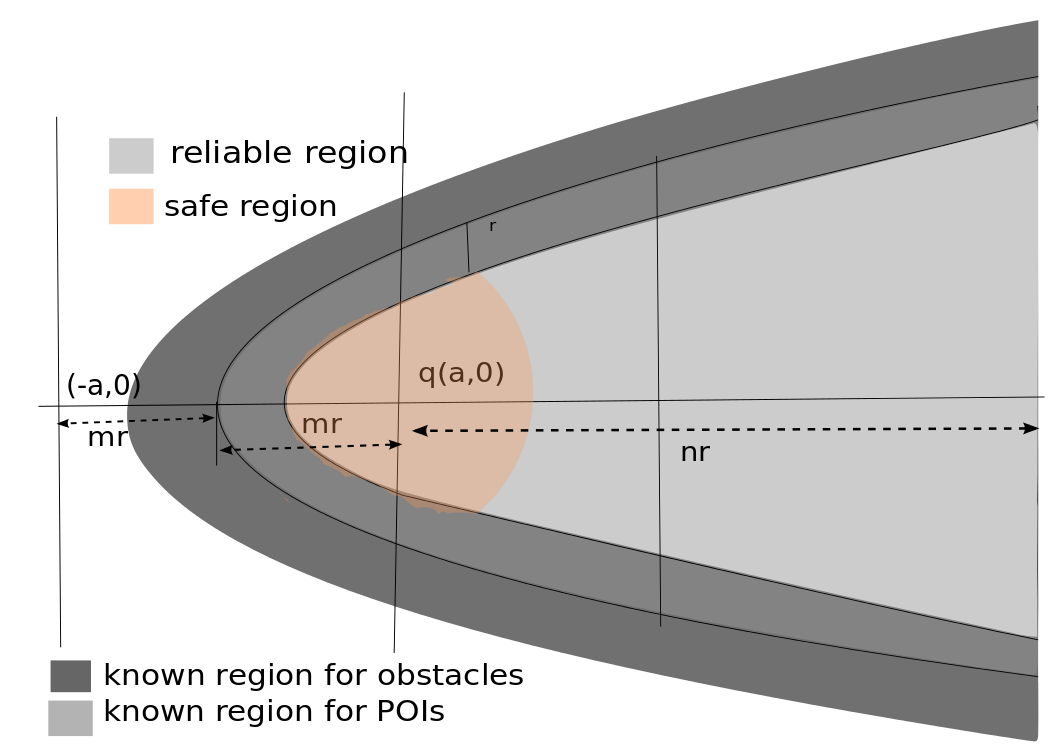
\includegraphics[width=\linewidth]{regions_def.png}
  \caption{Different regions}
  \label{fig:regions}
\end{figure}


\subsection{Bandwidth Saving Mode}
In this mode the main focus is to reduce the bandwidth of communication between the server and the client. This mode is designed to operate in three parts - \textit{client-initialization from server side}, \textit{alarm-configuration} and \textit{update on any minimal amount of location change}. The Algorithms \ref{GetAlarmablesFromServer}, \ref{ConfigAlarm}, \ref{ULC} show the algorithmic-steps for these three parts respectively.\\

The input to the client-initialization algorithm (Algorithm \ref{GetAlarmablesFromServer}) is the current location of the client $q$, query radius $r$, current velocity of the client $v$, path history as a set of straight lines $S$ = {$(m_1, c_1, l_1),$ $(m_2, c_2, l_2),$ $(m_3, c_3, l_3),$ ... $(m_n, c_n, l_n)$} and the last answer set $A_{prev}$ = {$q$, $u$, $m_p$, $m_o$, $n$}, where $u$ is the vertex of the . This algorithm makes the frequent queries more efficient and accurate and needs much less server communication.

% predictDirection getVertex varianceOfPath GetObstacleSet MakeVisGraph getCollisionPoint isPositivePoint pointOnStraightLine CheckNewPOI getCollisionPoint

In the following algorithms, \textsc{predictDirection}$(S)$ function returns a vector by inerpolating all the line segments given in a set $S$ as the client's path history. During the linear interpolation, the oldest path is given the minimum weight, while the later ones get the incrementally higher weights iventually giving the latest path segment the maximum weight and predicting the client's current direction most likely to be towards the latest paths.\\

The \textsc{getVertex}$(q, s_{dir})$ returns the vertex point $u$ of the parabola having focus at $q$ and the axis along the vector $s_{dir}$.\\

The function \textsc{varianceOfPath}$(S)$ returns a real number within the range [2, $\infty$) which is proportional to the variation of the client's path directions given the directed path segments in the set $S$. This value is assigned to the multiplier $m_p$ to construct the parabola $y^2 = 4*(m_p*r)*x$, since the more variation in the client's path requires more cross-section area of the known region parabola.\\

The \textsc{GetObstacleSet}$(q, m_o * r, n_p)$ returns all obstacles within the parabola $y^2 = 4*(m_o*r)*x$ which is again bounded by a straight line at $(n_p*r)$ distance from the focus $q$ and perpendicular to the axis of the parabola.\\

\textsc{getCollisionPoint}$(O, q, m_o, r, n_o)$ checks any collision of any of the obstales from the set $O$ with the parabola $y^2 = 4 * (m_o * r) * x$ and also the bounding straight line at distance $(n_o*r)$ from the focus $q$ and perpendicular to the axis of the parabola. Then it returns an all negative point if there is no collision, otherwise returns a positive point in the space. The \textsc{isPositivePoint}($p$) reutrns true for the point $p$ to be positive, otherwise returns false. Again, the function \textsc{pointOnStraightLine} ($p, n, r, q$) returns true if the point $p$ is on the straight line at distance $(n*r)$ from the focus $q$ and perpendicular to the axis of the parabola.\\

In this algorithm, \textsc{AttachToVisGraph}$(V_G, P, O)$ function adds the POIs and obstacles in the sets $P$ and $O$ respectively to the provided visibility graph $V_G$, so that minimal re-computation is needed.\\

The output of the Algorithm \ref{GetAlarmablesFromServer} is an answer set $A$ which consists of the radius of the known regions of POIs and obstacles ($r_{kp}$ and $r_{ko}$ respectively), the set $O$ of all obstacles within radius $r_{ko}$ and the set of all POIs within radius $r_{kp}$ centring $q$. Since it is a bandwidth saving mode, the visibility graph is not sent to the client as long as it can be computed using the existing data in the client side.\\

\begin{algorithm}
\caption{\textsc{QueryAlarmables}($q, r, v, S, A_{prev}$)}
\label{GetAlarmablesFromServer}
%\begin{algorithmic}[2]
%\Procedure{GetAlarmablesFromServer}{}

    \SetKwInOut{Input}{Input}
    \SetKwInOut{Output}{Output}
    \Input{Query point $q$, query radius $r$, velocity $v$, path history as a set of straight lines $S$, last answer set $A_{prev}$}
    \Output{The answer set, $A \gets \left\{ {q, u, m_p, n_p, m_o, n_o, P, O}\right\}$}
    
	 $s_{dir} \gets \textsc{predictDirection}(S)$ \;
	 $u \gets \textsc{getVertex}(q, s_{dir})$ \;
	 $m_p \gets \textsc{varianceOfPath}(S)$ \;
	 $n_p \gets ln( e + v )$ \;
	 
	 $O \gets \textsc{GetObstacleSet}(q, m_p * r, n_p)$ \;
	 $V_G \gets \textsc{MakeVisGraph}(P, O)$ \;
	 $m_o \gets m_p$ \;
	 $n_o \gets n_p$ \;
	 $p_{col} \gets \textsc{getCollisionPoint}(O, q, m_o, r, n_o)$ \;
	 \While { \textsc{isPositivePoint}$(p_{col})$ } {
	 	$O' \gets \emptyset$ \;
	 	$P' \gets \emptyset$ \;
	 	$b \gets \textsc{pointOnStraightLine} (p_{col}, n_o, r, q)$
	 	\If{$b$}{
			$O' \gets \textsc{GetObstacleSet}(q, u, m_o * r, n_o+1 )$ \;
			$P' \gets \textsc{CheckNewPOI}(q, u, m_o * r, n_o+1 )$ \;
			$n_o \gets (n_o + 1)$ \;
		}
		\Else{
			$O' \gets \textsc{GetObstacleSet}(q, u, (m_o+1) * r, n_o )$ \;
			$P' \gets \textsc{CheckNewPOI}(q, u, (m_o+1) * r, n_o )$ \;
			$m_o \gets (m_o + 1)$ \;
		}
		
		\If{$\left\vert{P'}\right\vert > \left\vert{P}\right\vert $}{
			$P \gets P'$ \;
			\If{$b$}{
				$m_p \gets (m_p+1) $\;
			}
			\Else{
				$n_p \gets (n_p+1) $\;
			}
	 		$V_G \gets \textsc{AttachToVisGraph}(V_G, P'-P, O'-O)$ 
		}
		$O \gets O'$ \;
	 	$p_{col} \gets \textsc{getCollisionPoint}(O, q, m_o, r, n_o)$ \;
	} \label{while}
	
	 \Return $A \gets \textsc{MakeAnswerSet}(q, u, m_p, n_p, m_o, n_o, P, O)$ 
%\EndProcedure
%\end{algorithmic}
\end{algorithm}

The input to the Algorithm \ref{ConfigAlarm} is the current location of the client $q$ and the answer set got from the Algorithm \ref{ClientGetAlarmables}. This algorithm is also responsible for triggering an alarm to the client if the client is within the alarming distance of any POI.
\begin{algorithm}
\caption{\textsc{ConfigUpdate}($q, A$)}
\label{ConfigAlarm}
%\begin{algorithmic}[4]
%\Procedure{ConfigAlarm}{}

    \SetKwInOut{Input}{Input}
    \SetKwInOut{Output}{Output}
    \Input{Query point $q$, answer set $A$}
    
    $P \gets GetPOIs(V_G)$\;
    $O \gets GetObstacles(V_G)$\;
    
    \ForEach{$p_i \in P$}{
    		$p_i.d_O \gets dist_O(q, p_i)$\;
    		\If{$p_i.d_O \leqslant r$}{
    			$\textsc{AlarmUser}(p_i)$\;
    		}
    		\ElseIf{$p_i.d_E<r_{safe}$ and $\textsc{isPathInside}(q, p_i, r_{safe}, V_G)$}{
    			$r_{safe} \gets p_i.d_E$ \;
    		}
    }
    \Return $r_{safe}$

%\EndProcedure
%\end{algorithmic}
\end{algorithm}

In this algorithm, the visibility graph is computed using the answer sets $P$ and $O$ got as return of the \ref{GetAlarmablesFromServer} from the server side.

%
%\begin{figure*}[!htb]
%\minipage{0.32\textwidth}
%  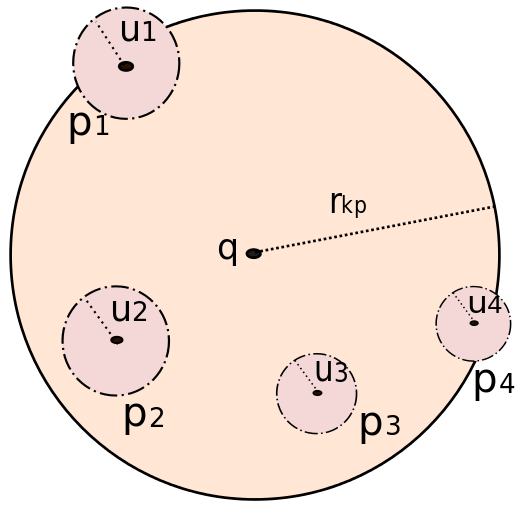
\includegraphics[width=\linewidth]{poi.png}
%  \caption{Retrieved POIs within $r_{kp}$ centring $q$}\label{fig:poi}
%\endminipage\hfill
%\minipage{0.32\textwidth}
%  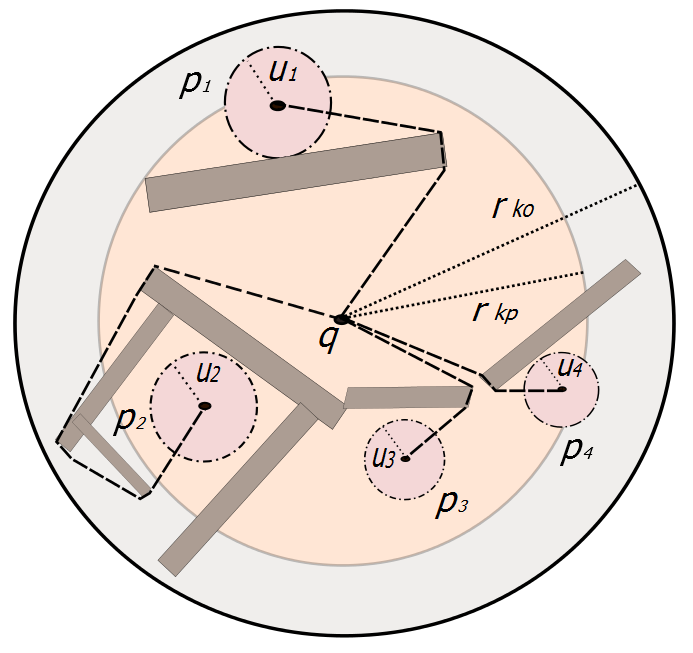
\includegraphics[width=\linewidth]{poi_obs_path.png}
%  \caption{Generated $V_G$}\label{fig:poi_obs_path}
%\endminipage\hfill
%\minipage{0.32\textwidth}%
%  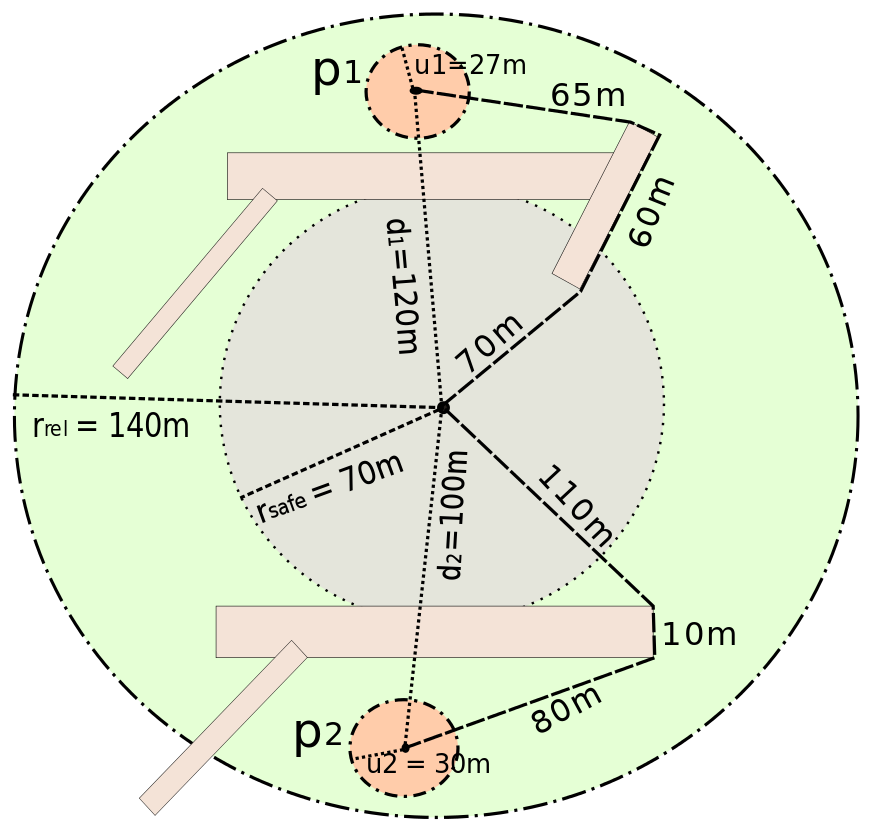
\includegraphics[width=\linewidth]{safe_region.png}
%  \caption{Safe Region Calculation}\label{fig:safe_region}
%\endminipage
%\end{figure*}
%%Figure \ref{fig:safe_region} Safe region Computation


The input to the algorithm \ref{ULC} is the current location of the client $q$, the radius of the safe region($r_{safe}$) and finally the already computed answer set $A$. The output of the algorithm is the minimum distance $d_u$ to trigger this algorithm the next time.

\begin{algorithm}
\caption{\textsc{UpdateOnLocChange}($q, r_{safe}, r_{rel}, A$)}
\label{ULC}
%\begin{algorithmic}[5]
%\Procedure{UpdateAlarm}{}

    \SetKwInOut{Input}{Input}
    \SetKwInOut{Output}{Output}
    \Input{$q, r_{safe}, A$}
    \Output{$d_u$}
    
    \If{$\textsc{isOutsideReliableregion(q, A)}$}{
    		$A \gets \textsc{QueryAlarmables}(q, d_q)$ \;
    		$r_{safe} \gets $ \textsc{ConfigAlarm}($q, A$) \;
    }
    
    \If{$d_q > r_{safe}$}{
    		$r_{safe} \gets $ \textsc{ConfigAlarm}($q, A$) \;
    }
    
    \Return $d_u \gets r_{safe}$

%\EndProcedure
%\end{algorithmic}
\end{algorithm}

\subsection{Computational Cost Saving Mode}
The algorithms run in this mode almost similarly as in the "\textit{Bandwidth Saving Mode}" with all the 3 described parts - \textit{client-initialization from server side}, \textit{alarm-configuration} and \textit{update on any minimal amount of location change} as demonstrated in the Algorithms \ref{ClientGetAlarmables}, \ref{ConfigAlarm}, \ref{ULC}.

However, the main difference with the previously descried mode from this mode is - the Algorithm \ref{GetAlarmablesFromServer} returning the computed $V_G$ as another element of the answer set $A$ from the server side and the algorithm \ref{ConfigAlarm} not reconstructing this $V_G$ in the client side during running the Algorithm \ref{ConfigAlarm}, whereas the Algorithm \ref{ULC} remains all the same.

Therefore, an $O(n^2)$ computation overhead for computing the $V_G$ is saved in the client-side in cost of a one-time communication overhead in transferring the $V_G$ in the Algorithm \ref{GetAlarmablesFromServer}.\\

%The above described approach can be depicted with some suitable examples as presented in the Figures \ref{fig:poi}, \ref{fig:poi_obs_path} and \ref{fig:safe_region}.\\
%
%In figure \ref{fig:poi} an example scenario is put as if 3 POIs $p_1, p_2,$ and $p_3$ are retrieved and in the figure \ref{fig:poi_obs_path} the same case is shown as if the algorithm \ref{ClientGetAlarmables} has returned the constructed visibility-graph $V_G$ along with the set of POIs $P$, obstacles $O$ and the radius of the POIs' known region $r_{kp}$ and that of the obstacles' known region $r_{ko}$.\\
%
%In the Figure \ref{fig:safe_region}, a critical case for the Algorithm \ref{ConfigAlarm} is demonstrated regarding the calculation of the safe region.
%
%During the for-loop at line no. 4 of the algorithm \ref{ConfigAlarm}, the safe-region's radius is calculated to be,
%\\$r_{safe} = min( (65+60+70)-27, (110+10+80)-30 ) = 168m$, whereas the safe-region is about to include both the POIs along with their whole path in the visibility graph $V_G$ from the center $q$ and also without any of them within their alarming zone. In this case as per the definition \ref{def:safe_region} , no calculation would be done to alarm the client even if s/he enters within any of the POI's alarming zone. To narrow down this false safe-region for the sake of accuracy, the condition of line no. 9 inside the foreach-loop gets true and the radius is modified as $r_{safe} = min(168, 120-27) = 93m$ for $p_1$ and in the second and final iteration for $p_2$, $r_{safe} = min( 93, 100-30) = 70m$.

%\subsection{Proof of Correctness}
%The following proved facts bear the proof of accuracy and completeness of our final algorithms \ref{ClientGetAlarmables}, \ref{ConfigAlarm} and \ref{ULC}.\\
%In the algorithm \ref{ClientGetAlarmables}, the fact that the incremental-search will find at least 1 POI and stop the increment to get a fixed $r_{kp}$ within finite time follows from the incremental search algorithm given the fact that the POI data-set is not empty.
%\\One more fact is to be proved to guarantee the accuracy and completeness of the algorithm \ref{ClientGetAlarmables} as - the while loop at line \ref{while} runs for a finite amount of time.
%
%\begin{proof}
%If there's no unreachable POI or no/single collision between any obstacle and the perimeter of the POIs' known region, then the loop will terminate immediately.
%\\If there is any totally unreachable POI, it must be surrounded by a series of obstacles, which will certainly cause no collision (in case that all obstacles are already inside the known region) or more than one collision (in case that some parts of the series of the obstacles are inside the known region) with the perimeter of the known region. So, the second clause will be false and the loop will terminate.
%\\Finally, if there is any unreachable POI which can be reached by retrieving an extended set of obstacles, then it will be done and checked inside the loop and then loop will finish its purpose within finite time.
%\end{proof}
%
%\textbf{No computation is needed to accurately give alarm while the user is inside the safe region.}\\
%
%\begin{proof}
%\textit{Case 1}: When the path to a POI is a straight line: 
%In this case the claim is trivial to prove. We take $min( D_i - U_i )$ as the radius of safe region. Suppose there is a POI $P$ with alarming distance $U$. The radius of the safe region is $r$. and the users current position is $p'$. Suppose for contradiction an alarm should be triggered to the user for $P$ in his current position $p'$. Then, $|p-p'|>(D-U)$. But as the user is within the safe region, $|p-p'|<r$ . But that mean, $r>|D-U|$ which is a contradiction because the algorithm \ref{ConfigAlarm} chooses the minimum between all $(D_i - U_i )$.
%\textit{Case 2:} When the path to a POI is not a straight line: 
%In this case there is an obstacle in the path to the POI. There can be two cases, 
%a. the safe region contains the full path to the obstructed POI 
%b. The safe region does not contain the full path to the obstructed POI.
%In case a, the algorithm \ref{ConfigAlarm} computes the minimum among the Euclidean distances of the POIs. As we know from the Euclidean lower bound property that the $dist_O(a,b) \geqslant dist_E(a,b)$, the proof follows from case 1. The safe region's radius will never over-assume the distance to the POI as it is considering the Euclidean distance.
%In case b, the algorithm \ref{ConfigAlarm} chooses the safe-region radius with the assumption that as the POI's full path is not the safe region, even if the user get's close to the POI in Euclidean Distance, Obstructed distance will always be higher.(Euclidean Lower Bound)
%\end{proof}
%
%\textbf{No query to the server has to be done to correctly give any alarm while the user is inside the reliable region}\\
%Recall from algorithms \ref{ClientGetAlarmables} and \ref{ConfigAlarm} that the minimum alarming distance among all the available POIs for the user is returned as $U_{min}$, which is used to reduce the POIs' known region's radius to the reliable region's radius as $r_{rel}$ = $r_{ko} - U_{max}$.
%
%\begin{proof}
%If the safe region is well inside the safe region, then this proof follows the 1st fact.
%The 3 procedures run simultaneously to give accurate alarm for the POIs inside the known region and so inside the reliable as well as the safe region.
%The proof is needed for any POI outside both the known regions.
%
%Let there be a POI outside both the known regions for which no alarm is triggered when the user gets inside its alarming distance $U_i$. 
%But meanwhile, the user must cross the reliable region because $r_{ko} - r_{rel} = U_{max} > U_i$ 
%So according to algorithm \ref{ULC}, algorithm \ref{ClientGetAlarmables} and \ref{ConfigAlarm} are re-run and the assumed POI must come inside the newly computed known regions and its alarm will be given accurately.
%Hence, there is a contradiction.
%Therefore, there is no POI outside the reliable region which may miss its alarm.
%So, the statement is proved.
%\end{proof}
%
%\textbf{The update procedure is run timely to re-calculate the answer set.}
%\begin{proof} 
%This claim follows trivially from the proof of the fact that - no computation is needed to accurately give alarm while the user is inside the safe region.
%\end{proof}
%

\section{Experiments}


\section{Conclusions}
This paragraph will end the body of this sample document.
Remember that you might still have Acknowledgments or
Appendices; brief samples of these
follow.  There is still the Bibliography to deal with; and
we will make a disclaimer about that here: with the exception
of the reference to the \LaTeX\ book, the citations in
this paper are to articles which have nothing to
do with the present subject and are used as
examples only.
%\end{document}  % This is where a 'short' article might terminate

%ACKNOWLEDGMENTS are optional
\section{Acknowledgments}
This section is optional; it is a location for you
to acknowledge grants, funding, editing assistance and
what have you.  In the present case, for example, the
authors would like to thank Gerald Murray of ACM for
his help in codifying this \textit{Author's Guide}
and the \textbf{.cls} and \textbf{.tex} files that it describes.


\bibliographystyle{plain}
\bibliography{lee}  
\appendix
%Appendix A
\section{Headings in Appendices}
The rules about hierarchical headings discussed above for
the body of the article are different in the appendices.
In the \textbf{appendix} environment, the command
\textbf{section} is used to
indicate the start of each Appendix, with alphabetic order
designation (i.e. the first is A, the second B, etc.) and
a title (if you include one).  So, if you need
hierarchical structure
\textit{within} an Appendix, start with \textbf{subsection} as the
highest level. Here is an outline of the body of this
document in Appendix-appropriate form:
\subsection{Introduction}
\subsection{The Body of the Paper}
\subsubsection{Type Changes and  Special Characters}
\subsubsection{Math Equations}
\paragraph{Inline (In-text) Equations}
\paragraph{Display Equations}
\subsubsection{Citations}
\subsubsection{Tables}
\subsubsection{Figures}
\subsubsection{Theorem-like Constructs}
\subsubsection*{A Caveat for the \TeX\ Expert}
\subsection{Conclusions}
\subsection{Acknowledgments}
\subsection{Additional Authors}
This section is inserted by \LaTeX; you do not insert it.
You just add the names and information in the
\texttt{{\char'134}additionalauthors} command at the start
of the document.
\subsection{References}
Generated by bibtex from your ~.bib file.  Run latex,
then bibtex, then latex twice (to resolve references)
to create the \cite{mur} ~.bbl file. \cite{roadalarm} Insert that ~.bbl file into
the .tex source file and comment out
the command \texttt{{\char'134}thebibliography}.
% This next section command marks the start of
% Appendix B, and does not continue the present hierarchy
\section{More Helps}
The sig-alternate.cls file itself is chock-full of succinct
and helpful comments.  If you consider yourself a moderately
experienced to expert user of \LaTeX, you may find reading
it useful but please remember not to change it.

\end{document}
